




\begin{figure}[t]
    \centering
    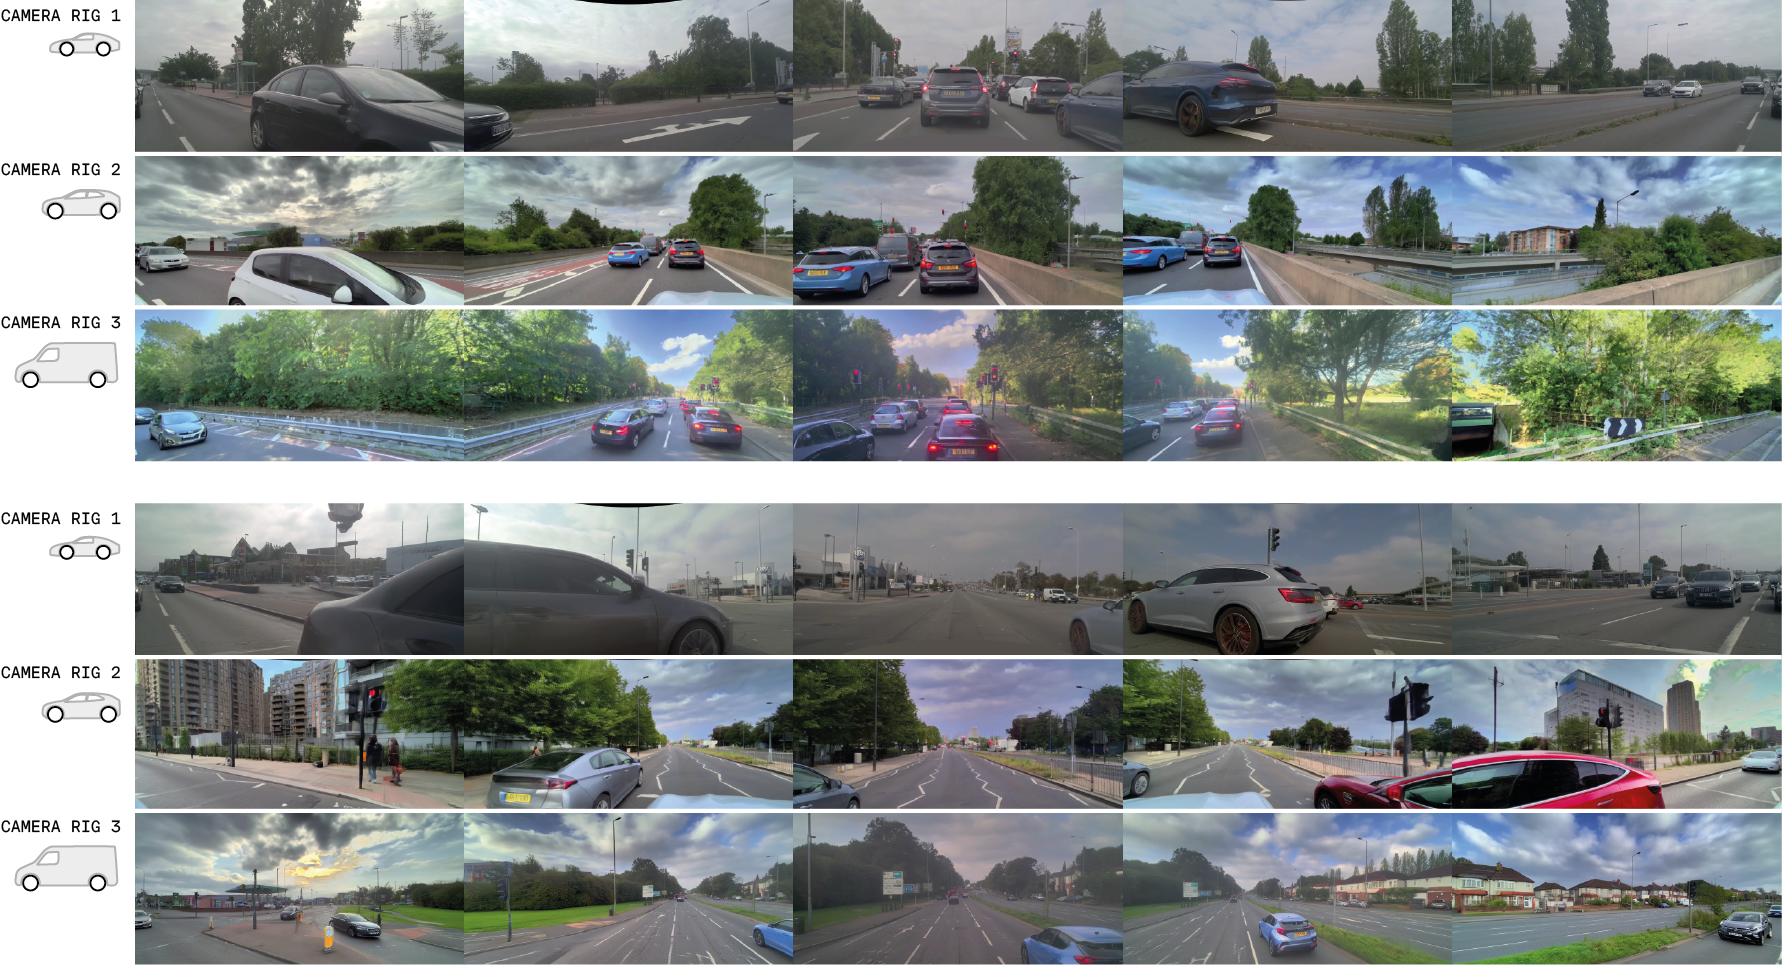
\includegraphics[width=1.0\textwidth]{Figures/platforms_v2.png}
    \caption{\textbf{Multi-rig video generation}. GAIA-2 supports various vehicle platforms and camera setups, maintaining spatial and temporal consistency. The two examples shown include camera arrangements from a sports car, an SUV, and a large van.}
    \label{fig:camera-rigs}
\end{figure}

\begin{figure}[t]
  \centering
  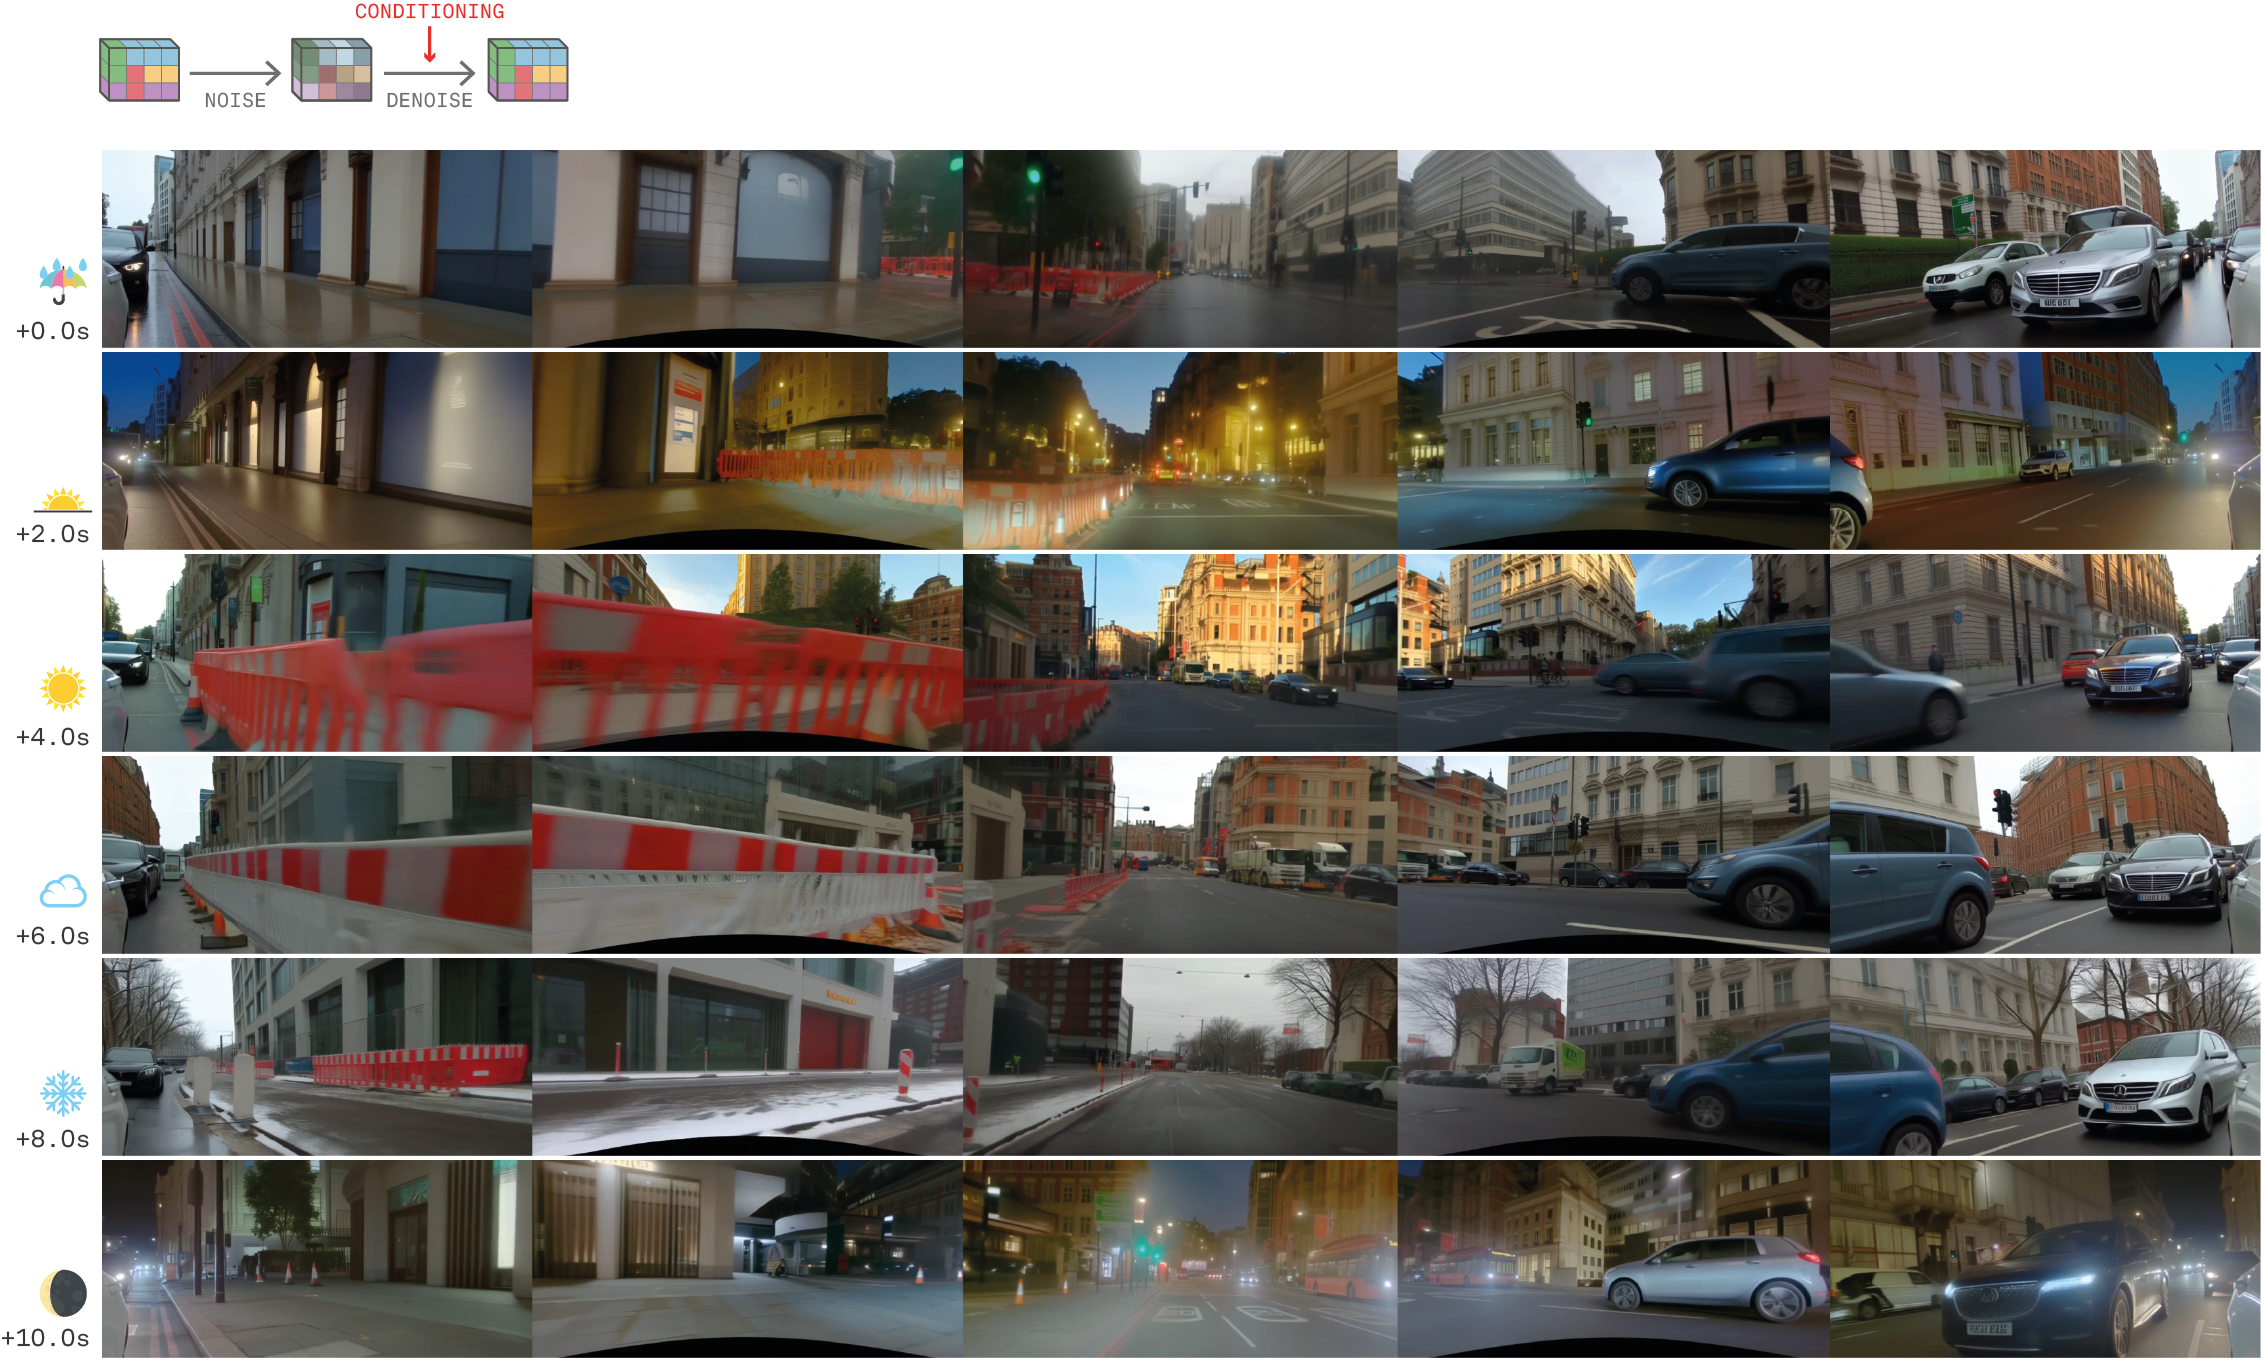
\includegraphics[width=1.0\textwidth]{Figures/noisedenoise.png}
  \caption{\textbf{Augmentation through partial noising.} By partially noising and denoising video frames, GAIA-2 transforms real video into diverse versions under different environmental settings, such as weather and time of day, while preserving semantic content and ego-actions.}
  \label{fig:noisedenoise}
\end{figure}

\begin{figure}[t]
  \centering
  \makebox[\textwidth][c]{%
    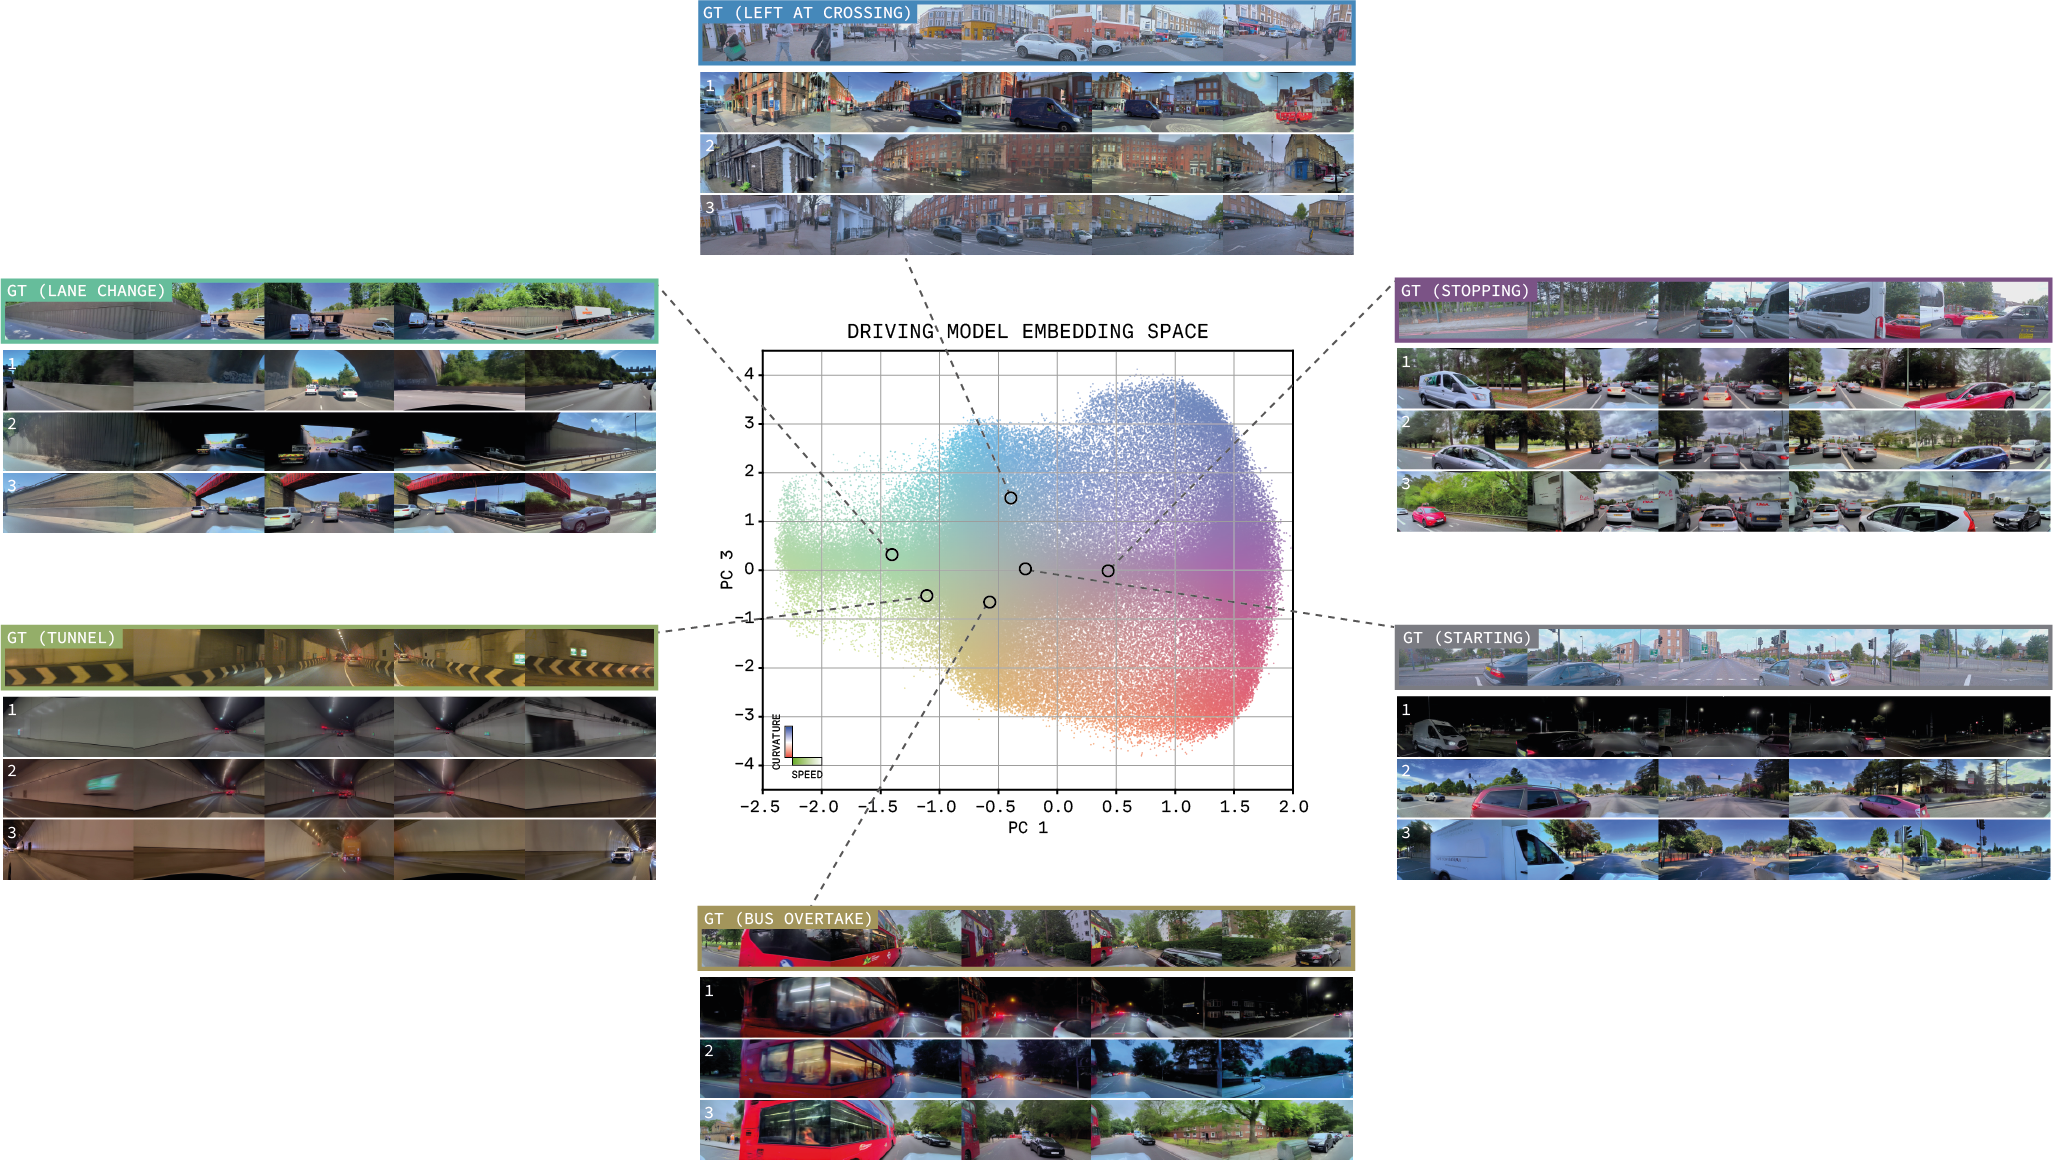
\includegraphics[width=1\textwidth]{Figures/gd_embedding_v2.png}
    }
  \caption{\textbf{Scenario embedding conditioning}. Scenario embeddings from a proprietary driving model enable GAIA-2 to generate diverse yet semantically consistent variations from real-world scenarios. For each scenario type the top row shows the real data the embedding is derived from, and the bottom three rows show synthetic variants of it, guided by the embedding as conditioning. We also optionally apply additional conditioning such as country, weather, time of day, or camera parameters to control diversity.}
  \label{fig:embeddings}
\end{figure}




\section{Results}
\label{section:results}

We evaluate GAIA-2 through qualitative examples and quantitative metrics that highlight its generative fidelity, controllability, and suitability for synthetic data generation in autonomous driving. A comprehensive set of generated video examples is available at \url{https://wayve.ai/thinking/gaia-2}.

\paragraph{Augmenting Real-World Data.}
GAIA-2 enables dataset augmentation through a range of techniques that allow for visual and contextual diversification of real-world sequences.


\subsection{Qualitative Examples}

\paragraph{Diverse Scenario Generation.}
GAIA-2 supports the generation of highly diverse driving scenarios, spanning multiple countries, weather conditions, times of day, and road layouts. In addition to structured conditioning via metadata, GAIA-2 can be guided by CLIP embeddings, allowing control over scene semantics not explicitly captured in labels. This includes geographic and environmental context such as urban, mountainous, or coastal scenes (\Cref{fig:clip}).

Furthermore, due to its exposure to varied camera configurations during training, GAIA-2 can simulate driving videos across different vehicle embodiments. By conditioning on camera parameters, it maintains spatial and temporal consistency across viewpoints for rigs mounted on sports cars, SUVs, and large vans (\Cref{fig:camera-rigs}).


\begin{itemize}
\item \textbf{Partial noise and denoise:} Latents derived from real videos are partially noised and then denoised under altered conditioning, such as different weather or lighting. This approach preserves semantics and ego motion while yielding diverse visual outputs (Figure~\ref{fig:noisedenoise}). We demonstrate the ability to modify environmental aspects of the scene while leaving core semantic and functional components as per the original. Essentially turning a single real-world example into multiple new scenarios: the same ego trajectory but visually diversified to take place during sunshine, rain, at sunset, at night, and in the snow.
\item \textbf{Scenario embeddings:} Scenario embeddings derived from our proprietary driving models give GAIA-2 the ability to generate multiple plausible variations from a single real-world example, providing many new examples of diverse yet contextually coherent synthetic data (\Cref{fig:embeddings}). Because the embedding space is meaningfully organized by the driving model, we are able to reliably generate scenarios that are semantically interpretable given their location in the embedding space, such as accelerating, decelerating, or overtaking other agents. By additionally conditioning on environmental factors, we can synthetically expand our dataset by increasing coverage across various conditions. By conditioning on different camera parameters, we can effectively replicate our corpus across any given vehicle platform.
\item \textbf{Action-based generation:} GAIA-2 can synthesize new scenes purely from ego-vehicle action trajectories. Given the speed and curvature profiles, it generates plausible visual contexts aligned with those dynamics, such as traffic light changes, braking behavior, or turning maneuvers (\Cref{fig:from-scratch-actions}). We show three examples: (1) conditioning on a `\textit{start from stopped}' speed profile, GAIA-2 generates plausible visual observations to fit those actions, in this case, a UK traffic light turning from red and amber to green; (2) conditioning on a `\textit{slow to a stop}' speed trajectory, GAIA-2 generates a scenario where the ego agent is slowing down behind a London taxi; and (3) conditioned on a strong leftward curvature and slow ramping speed, GAIA-2 generates a U-turn at a US intersection.
\end{itemize}








\begin{figure}[t]
  \centering
  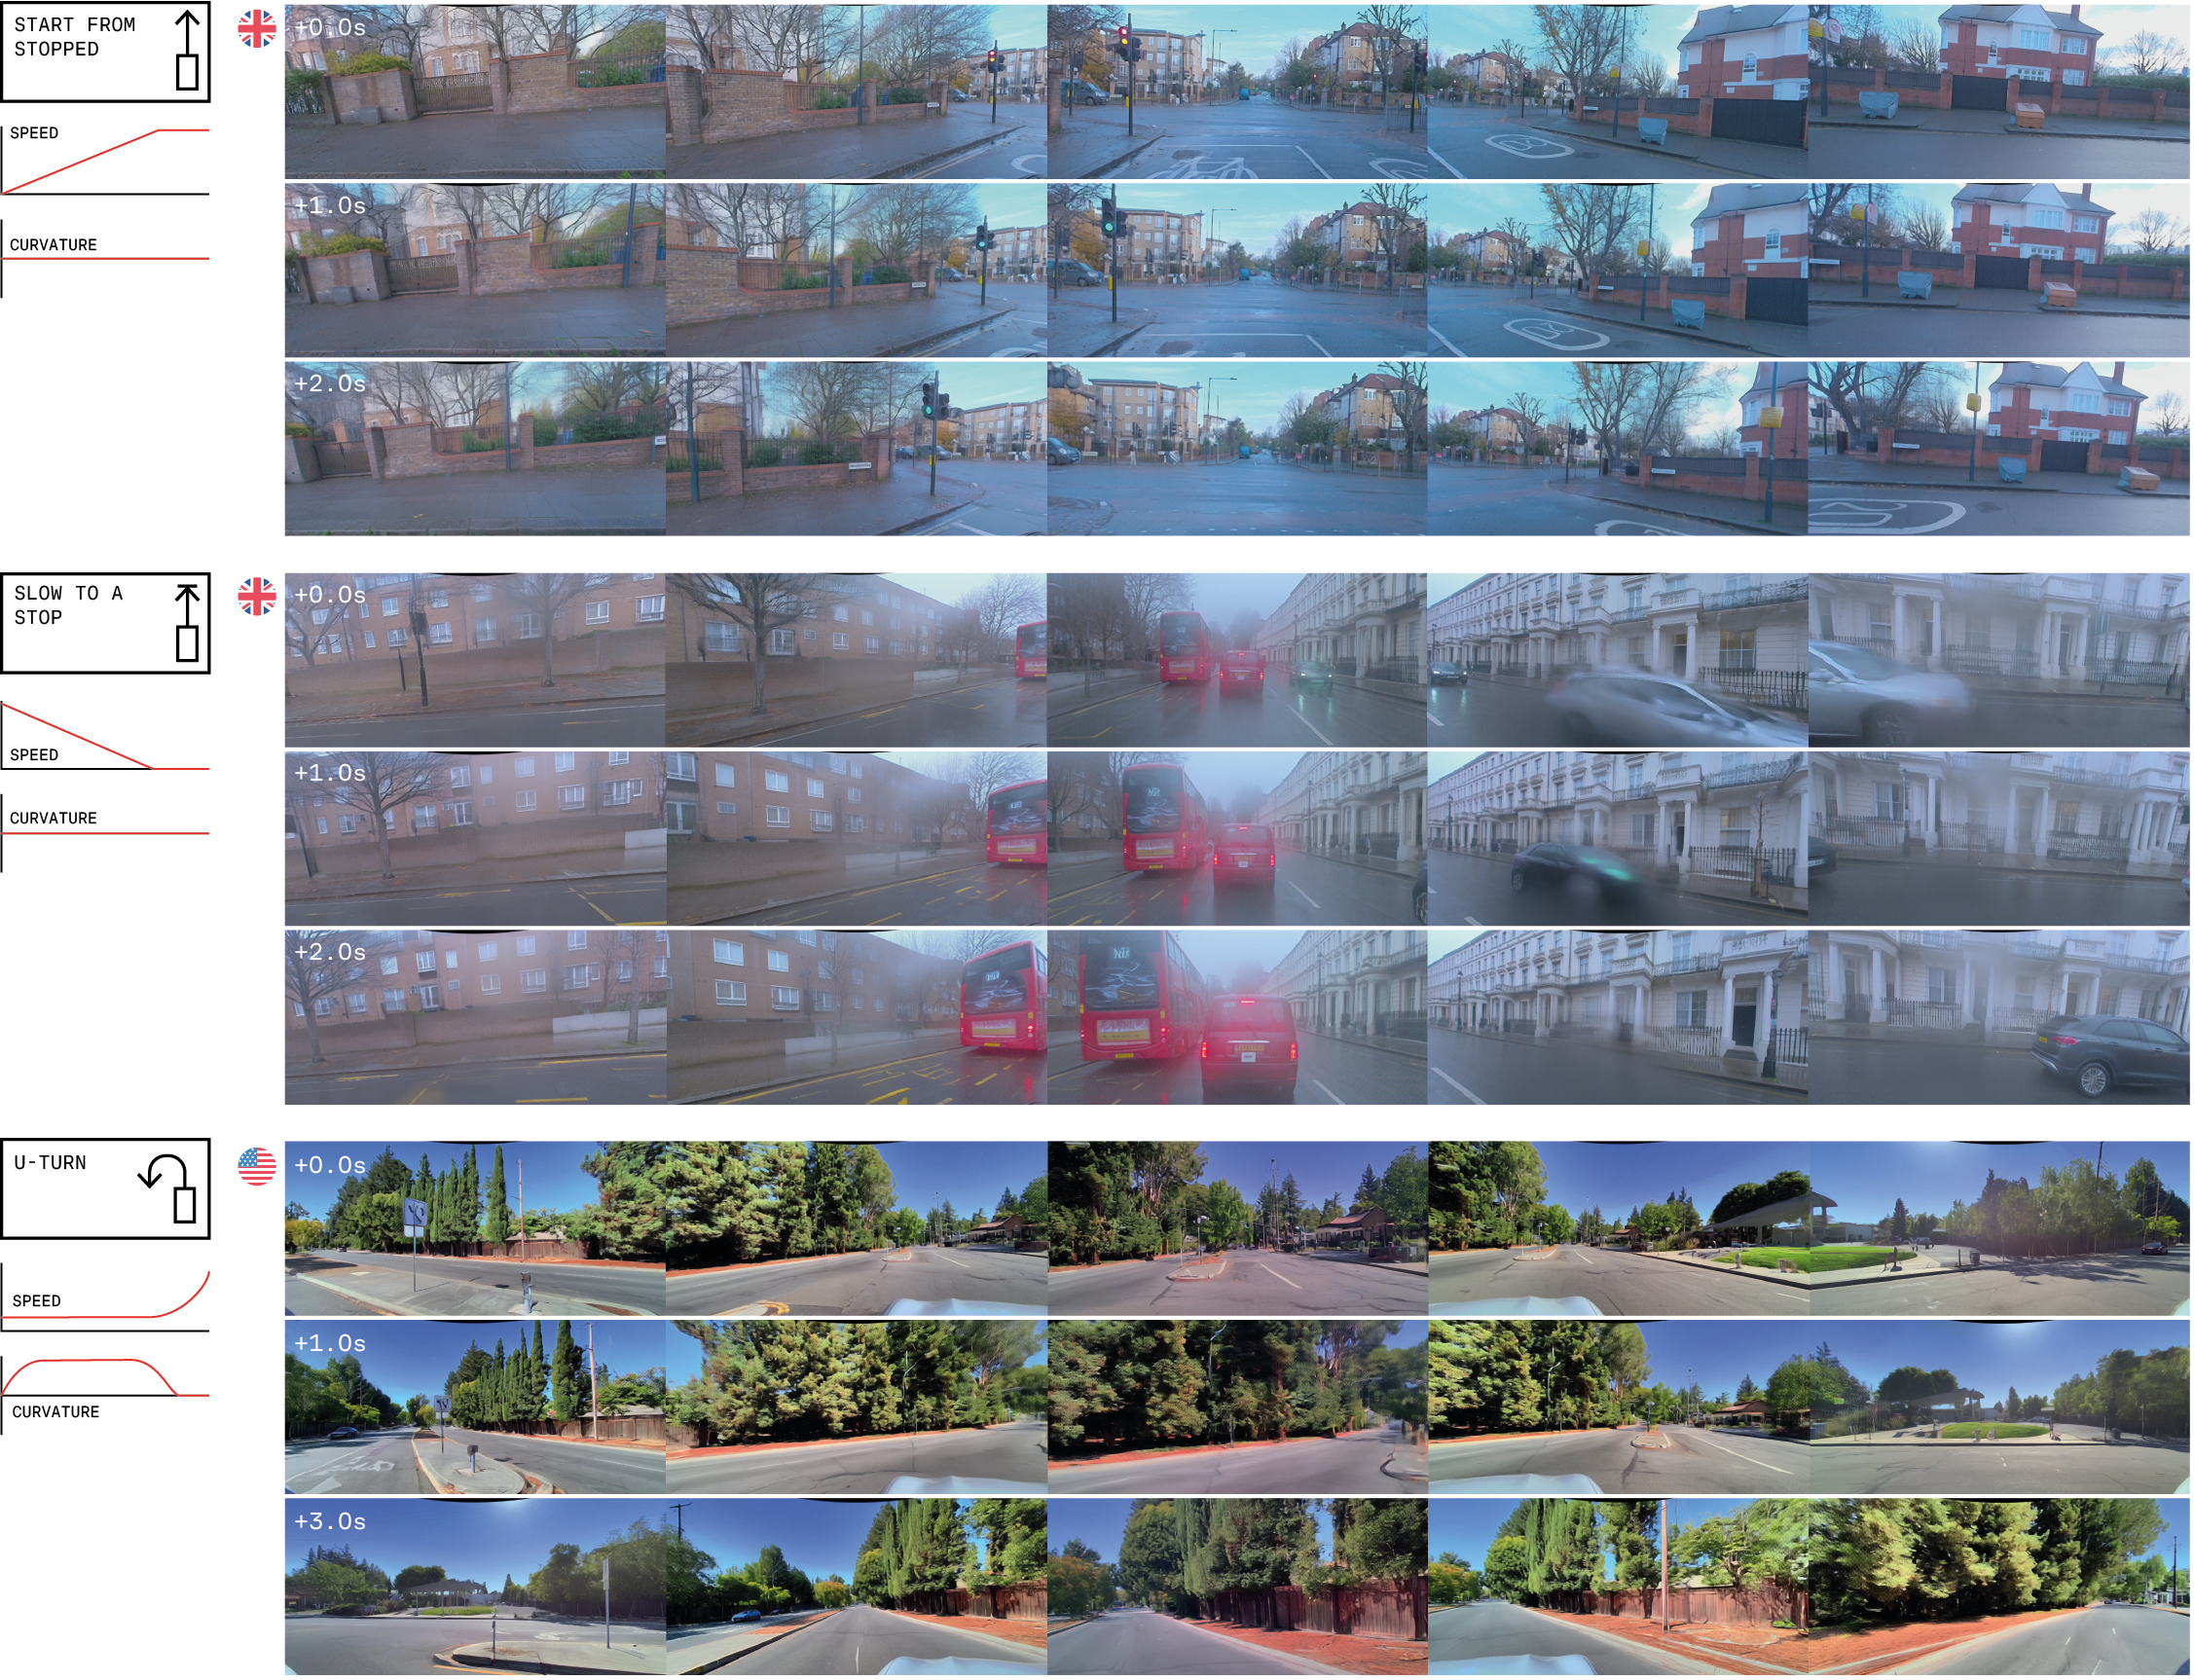
\includegraphics[width=1.0\textwidth]{Figures/actions_v2.png}
  \caption{\textbf{Action-based generation}. GAIA-2 synthesizes diverse scenes from specified speed and curvature profiles. Each scenario is contextually plausible, despite the original video inputs being dropped out.}
  \label{fig:from-scratch-actions}
\end{figure}

\paragraph{Generating Safety-Critical Scenarios.}
GAIA-2 is able to generate rare but safety-critical scenarios that would otherwise occur infrequently in the real world. We consider two classes of safety-critical situations: those caused by the ego agent, and those caused by other agents.
% 
\begin{itemize}
\item \textbf{Ego-vehicle induced scenarios:} By conditioning on extreme or unsafe ego-vehicle actions (e.g., abrupt steering into oncoming traffic), GAIA-2 generates realistic scenarios critical to testing autonomous system resilience under hazardous conditions (\Cref{fig:unsafe-actions} and \Cref{fig:ood}).
\item \textbf{Other-agent induced scenarios:} Using 3D bounding boxes conditioning, GAIA-2 precisely controls the placement and motion of other agents, creating scenarios involving aggressive driving behaviors, emergency braking, or hazardous crossings, crucial for testing reactive capabilities of autonomous systems (\Cref{fig:cuboids}).
\end{itemize}


\begin{figure}[t]
  \centering
  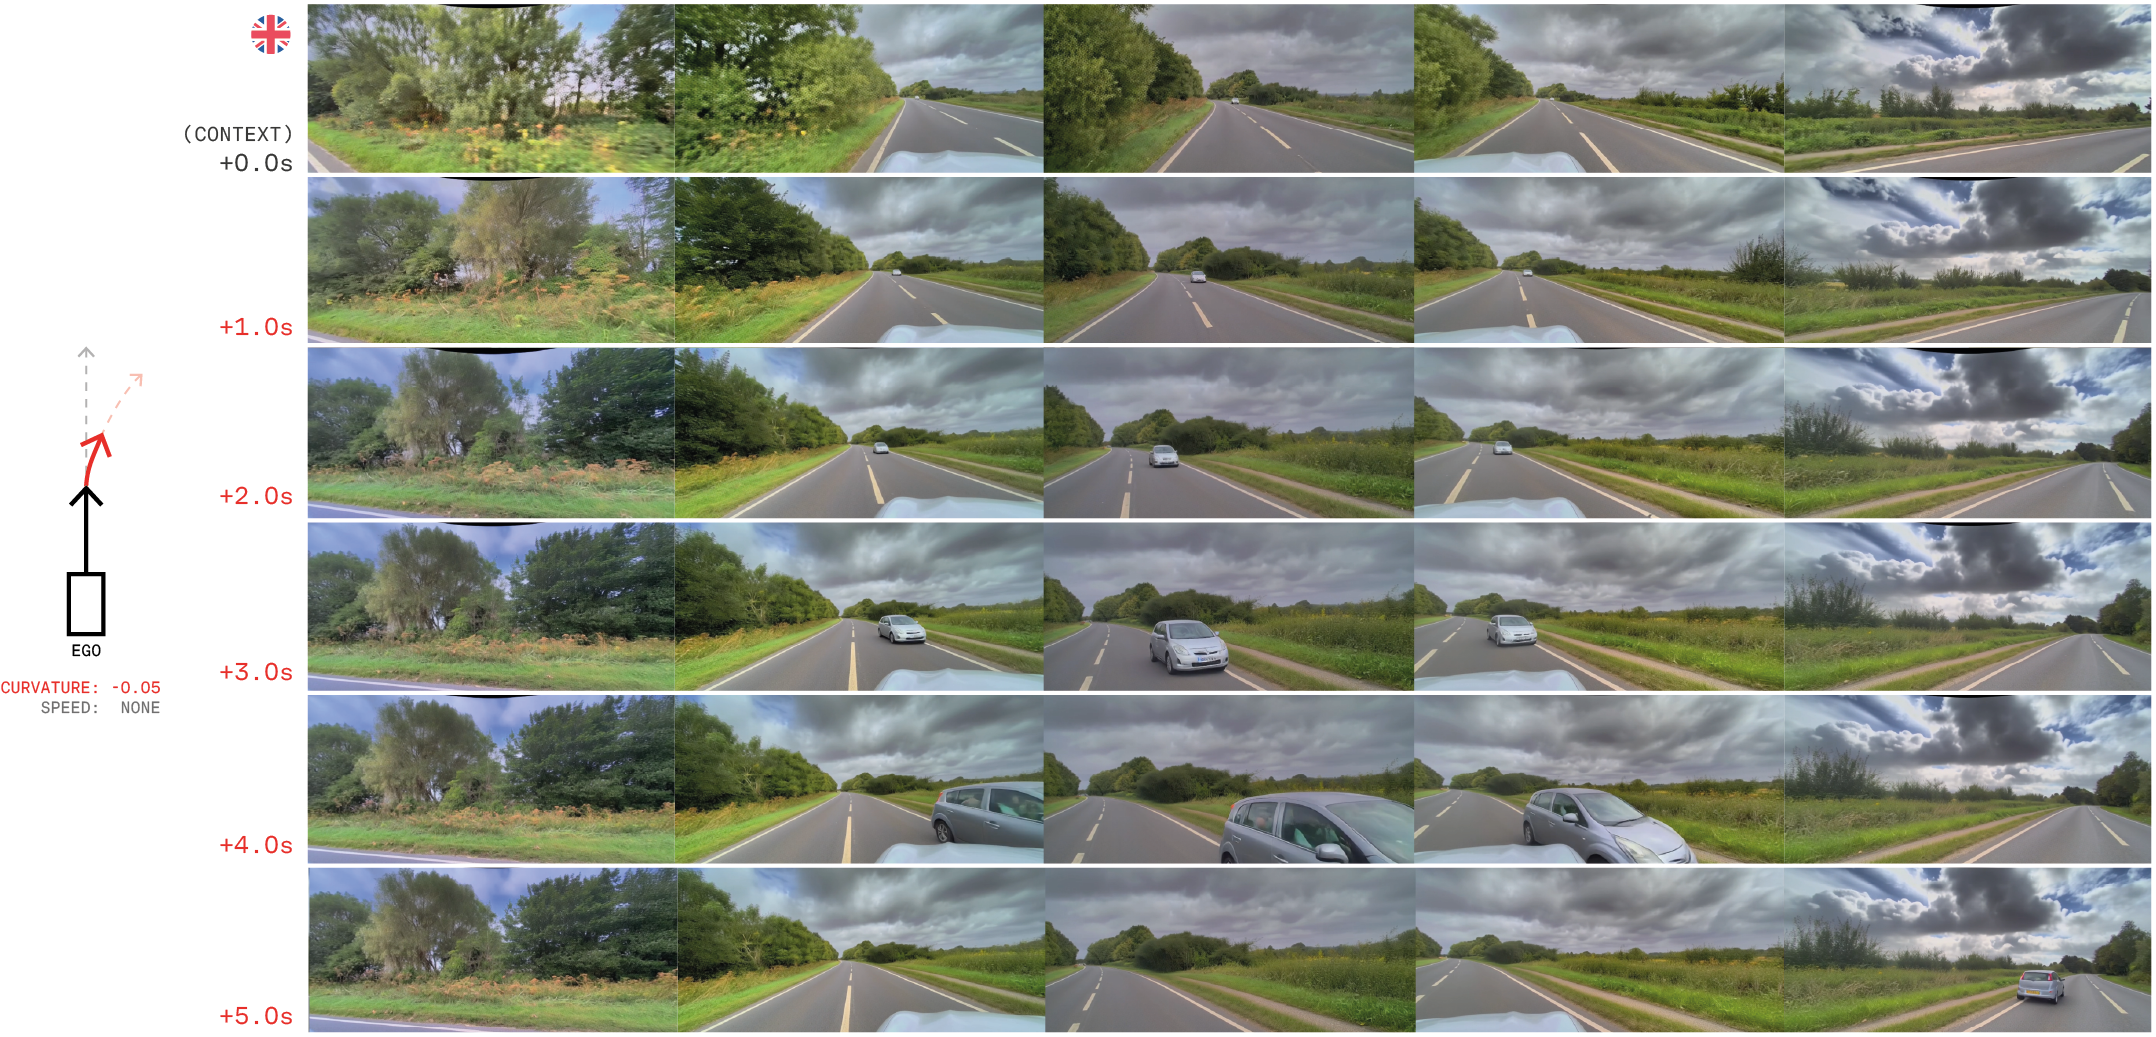
\includegraphics[width=1.0\textwidth]{Figures/unsafe_action.png}
  \caption{\textbf{Ego-induced safety-critical scenarios}. By applying unsafe action conditioning, GAIA-2 can generate hazardous situations, such as steering into oncoming traffic. We provide real video frames as context and GAIA-2 rolls out from these starting frames given some new action conditioning. In this example, we control the ego vehicle steering by conditioning on rightward curvature. We drop out speed so that GAIA-2 can generate multiple diverse outcomes. Note how the ego vehicle slows down while veering sharply into oncoming traffic. The oncoming vehicle swerves to avoid the ego vehicle.}
  \label{fig:unsafe-actions}
\end{figure}



\begin{figure}[t]
  \centering
  \makebox[\textwidth][c]{%
    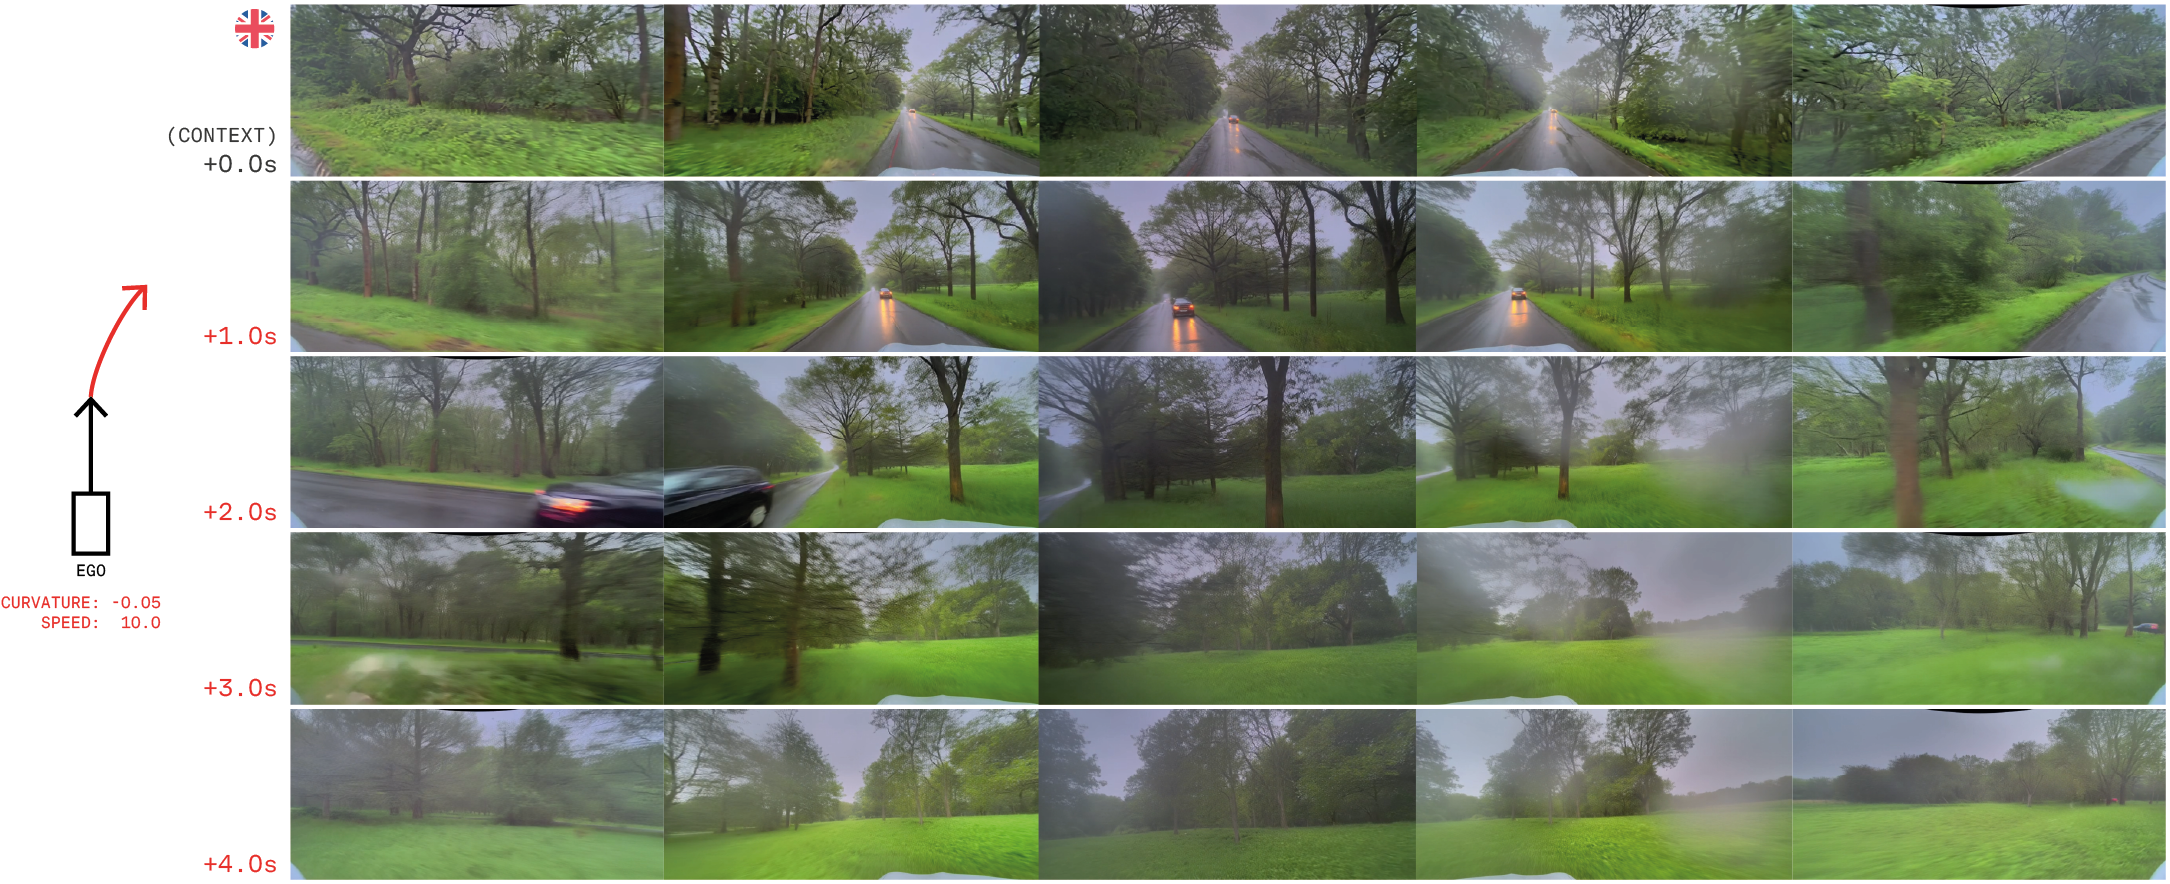
\includegraphics[width=1.0\textwidth]{Figures/ood_generalisation.png}%
  }
    \caption{\textbf{Extreme generalization behavior}. When conditioned on high speed and strong curvature, GAIA-2 extrapolates off-road trajectories, capturing rare behaviors like driving into fields or forests.} 
  \label{fig:ood}
\end{figure}


\begin{figure}[t]
  \centering
  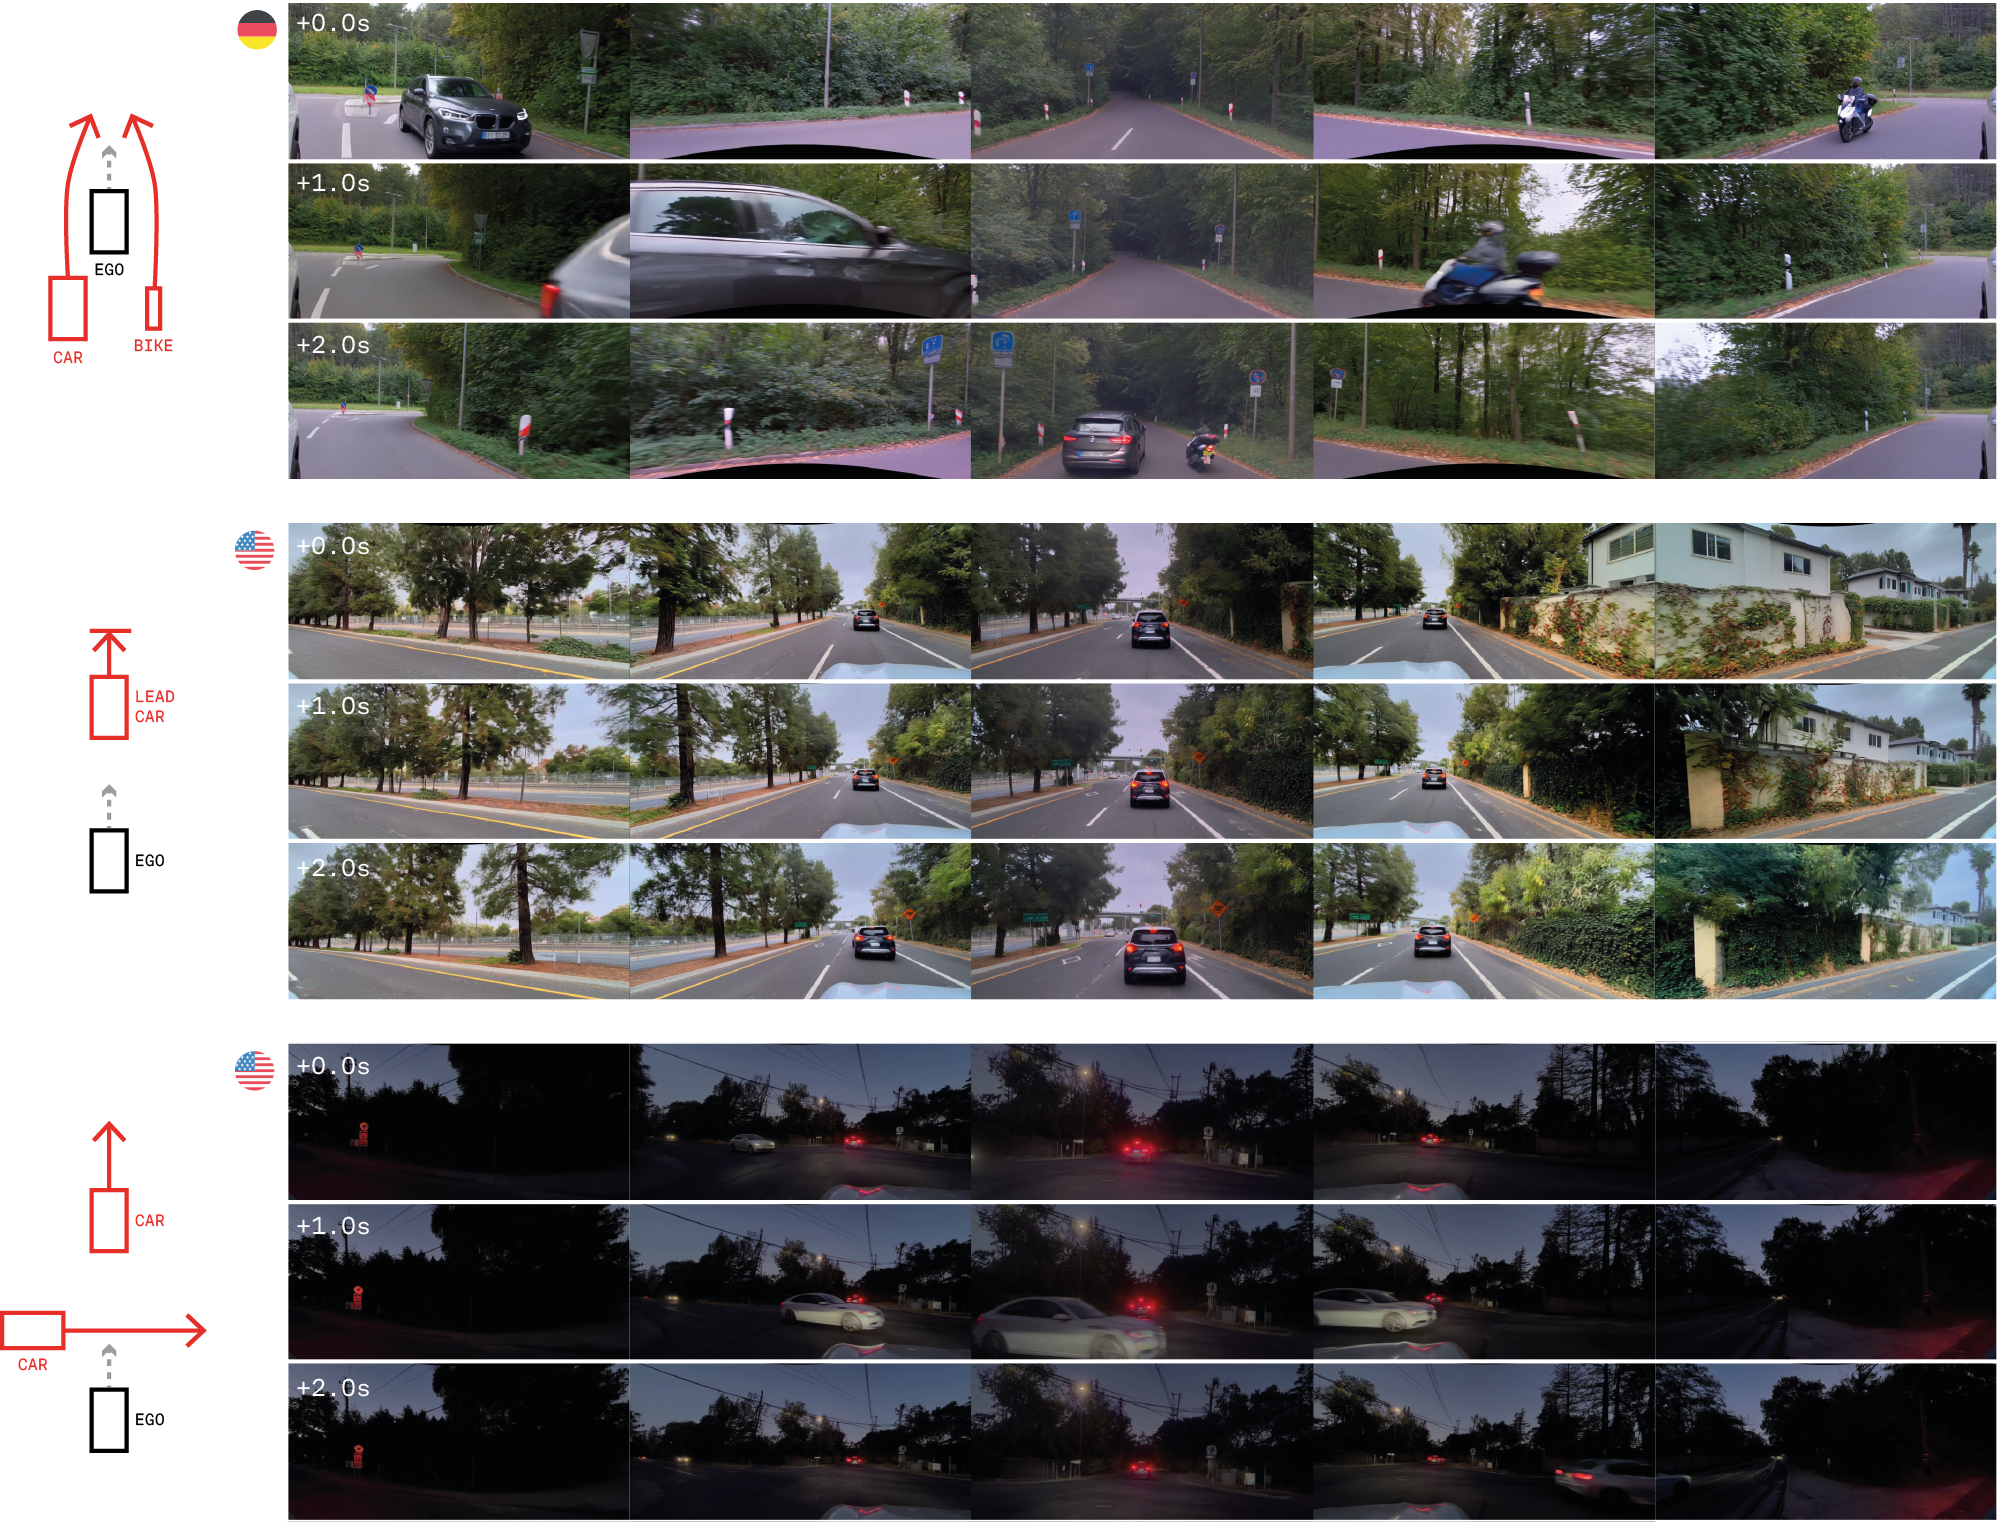
\includegraphics[width=1.0\textwidth]{Figures/cuboids.png}
  \caption{\textbf{Other-agent induced safety-critical scenarios}. 3D bounding box conditioning enables fine control over dynamic agents, allowing simulation of risky behaviors such as sudden braking, overtaking, or speeding through intersections.}
  \label{fig:cuboids}
\end{figure}

\paragraph{Inpainting.}
GAIA-2 supports spatial-temporal inpainting, enabling selective content editing. When provided with masked regions and corresponding agent-level conditioning, GAIA-2 inserts agents seamlessly into existing contexts without disrupting unrelated areas (\Cref{fig:inpainting}).

\begin{figure}[t]
  \centering
  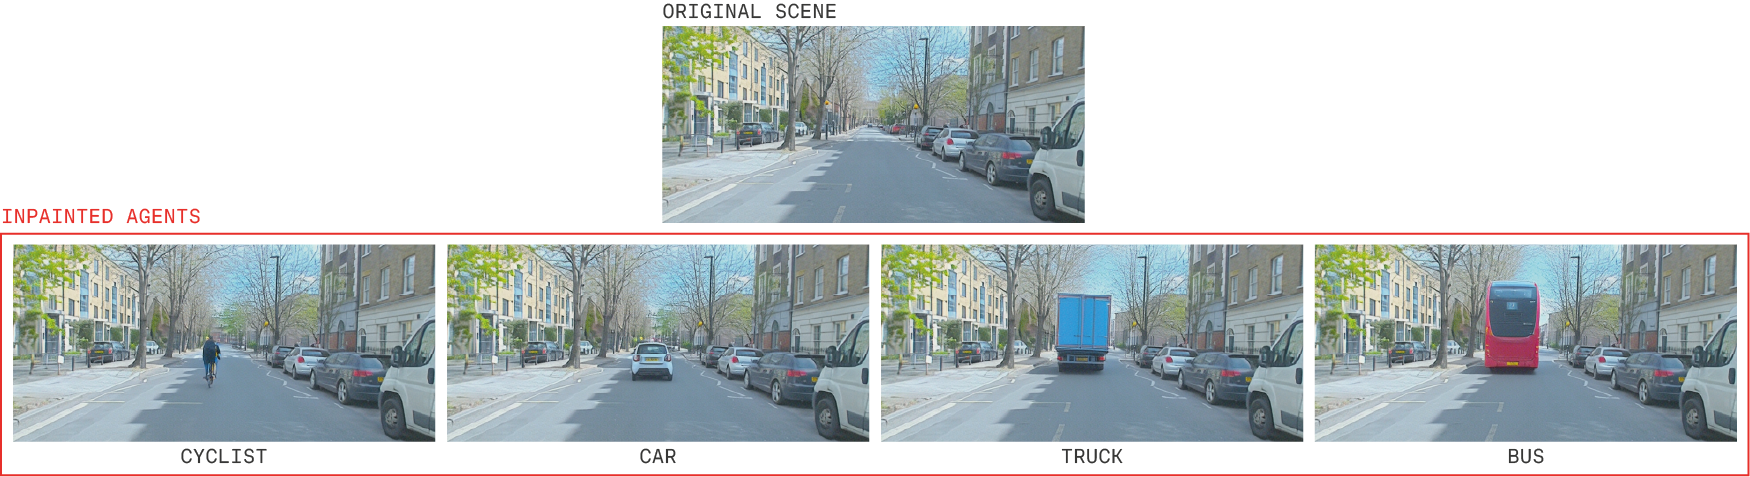
\includegraphics[width=1.0\textwidth]{Figures/inpainting.png}
  \caption{\textbf{Agent inpainting}. GAIA-2 can insert dynamic agents into masked regions of a video, guided by 3D bounding box conditioning. Background consistency and semantic realism are preserved.}
  \label{fig:inpainting}
\end{figure}

These qualitative results highlight GAIA-2’s ability to perform fine-grained and controllable video generation, supporting its use in scalable simulation and diverse scenario creation for autonomous systems.


\subsection{Metrics}
To quantitatively evaluate GAIA-2, we use a suite of metrics that assess visual fidelity, temporal consistency, and conditioning accuracy.

\paragraph{Visual Fidelity.}
Similarly to \cite{stein2023exposingflawsgenerativemodel}, we use the Frechet DINO Distance (FDD) and Frechet Inception Distance (FID) \cite{heusel2018ganstrainedtimescaleupdate} to measure the distance between the distributions of generated and real videos. The feature encoder is DINOv2 \cite{oquab2023dinov2} ViT-L/14, and the input images are bilinearly rescaled to a higher resolution $448 \times 952$ compared to $299 \times 299$ for InceptionV3 \cite{szegedy2015rethinkinginceptionarchitecturecomputer} in FID. We observe that FDD is less noisy than FID and saturates much later in training.

\paragraph{Temporal Consistency.} To evaluate the temporal consistency of the world model, we use the Frechet Video Motion Distance (FVMD) \cite{liu2024frechetvideomotiondistance}. This metric compares distributions of explicit key-point motion features for generated and ground-truth videos. We find this metric to be more aligned with human preferences for temporal consistency compared to FVD \cite{unterthiner18}.

% \paragraph{Geometric Consistency and Action Conditioning.} To evaluate geometric consistency of generated multi-camera videos we use Thresholded Symmetric Epipolar Distance (TSED) \cite{yu2023longtermphotometricconsistentnovel}. The metric evaluates geometric consistency between overlapping frames from different cameras or from same camera but at different timestamps. We use LoFTR \cite{sun2021loftrdetectorfreelocalfeature} to obtain key-point matches in overlapping images, then we compute fundamental matrix based on camera pose conditioning given to the world model, and finally compute the TSED metric to estimate how well the generated image pairs adhere to the camera pose conditioning. We use 2\% of image width as threshold to compute ratio of image pairs with acceptable geometric consistency.

% We use this method to evaluate action conditioning as well. To compute future camera poses we propagate the pose at current timestamp using vehicle trajectory specified in action conditioning. As we only can use static scene to compute geometric consistency between present and future frame, we exclude dynamic object key-points using OneFormer \cite{jain2022oneformertransformerruleuniversal} segmentation model.Dy

\begin{figure}[t]
    \centering
    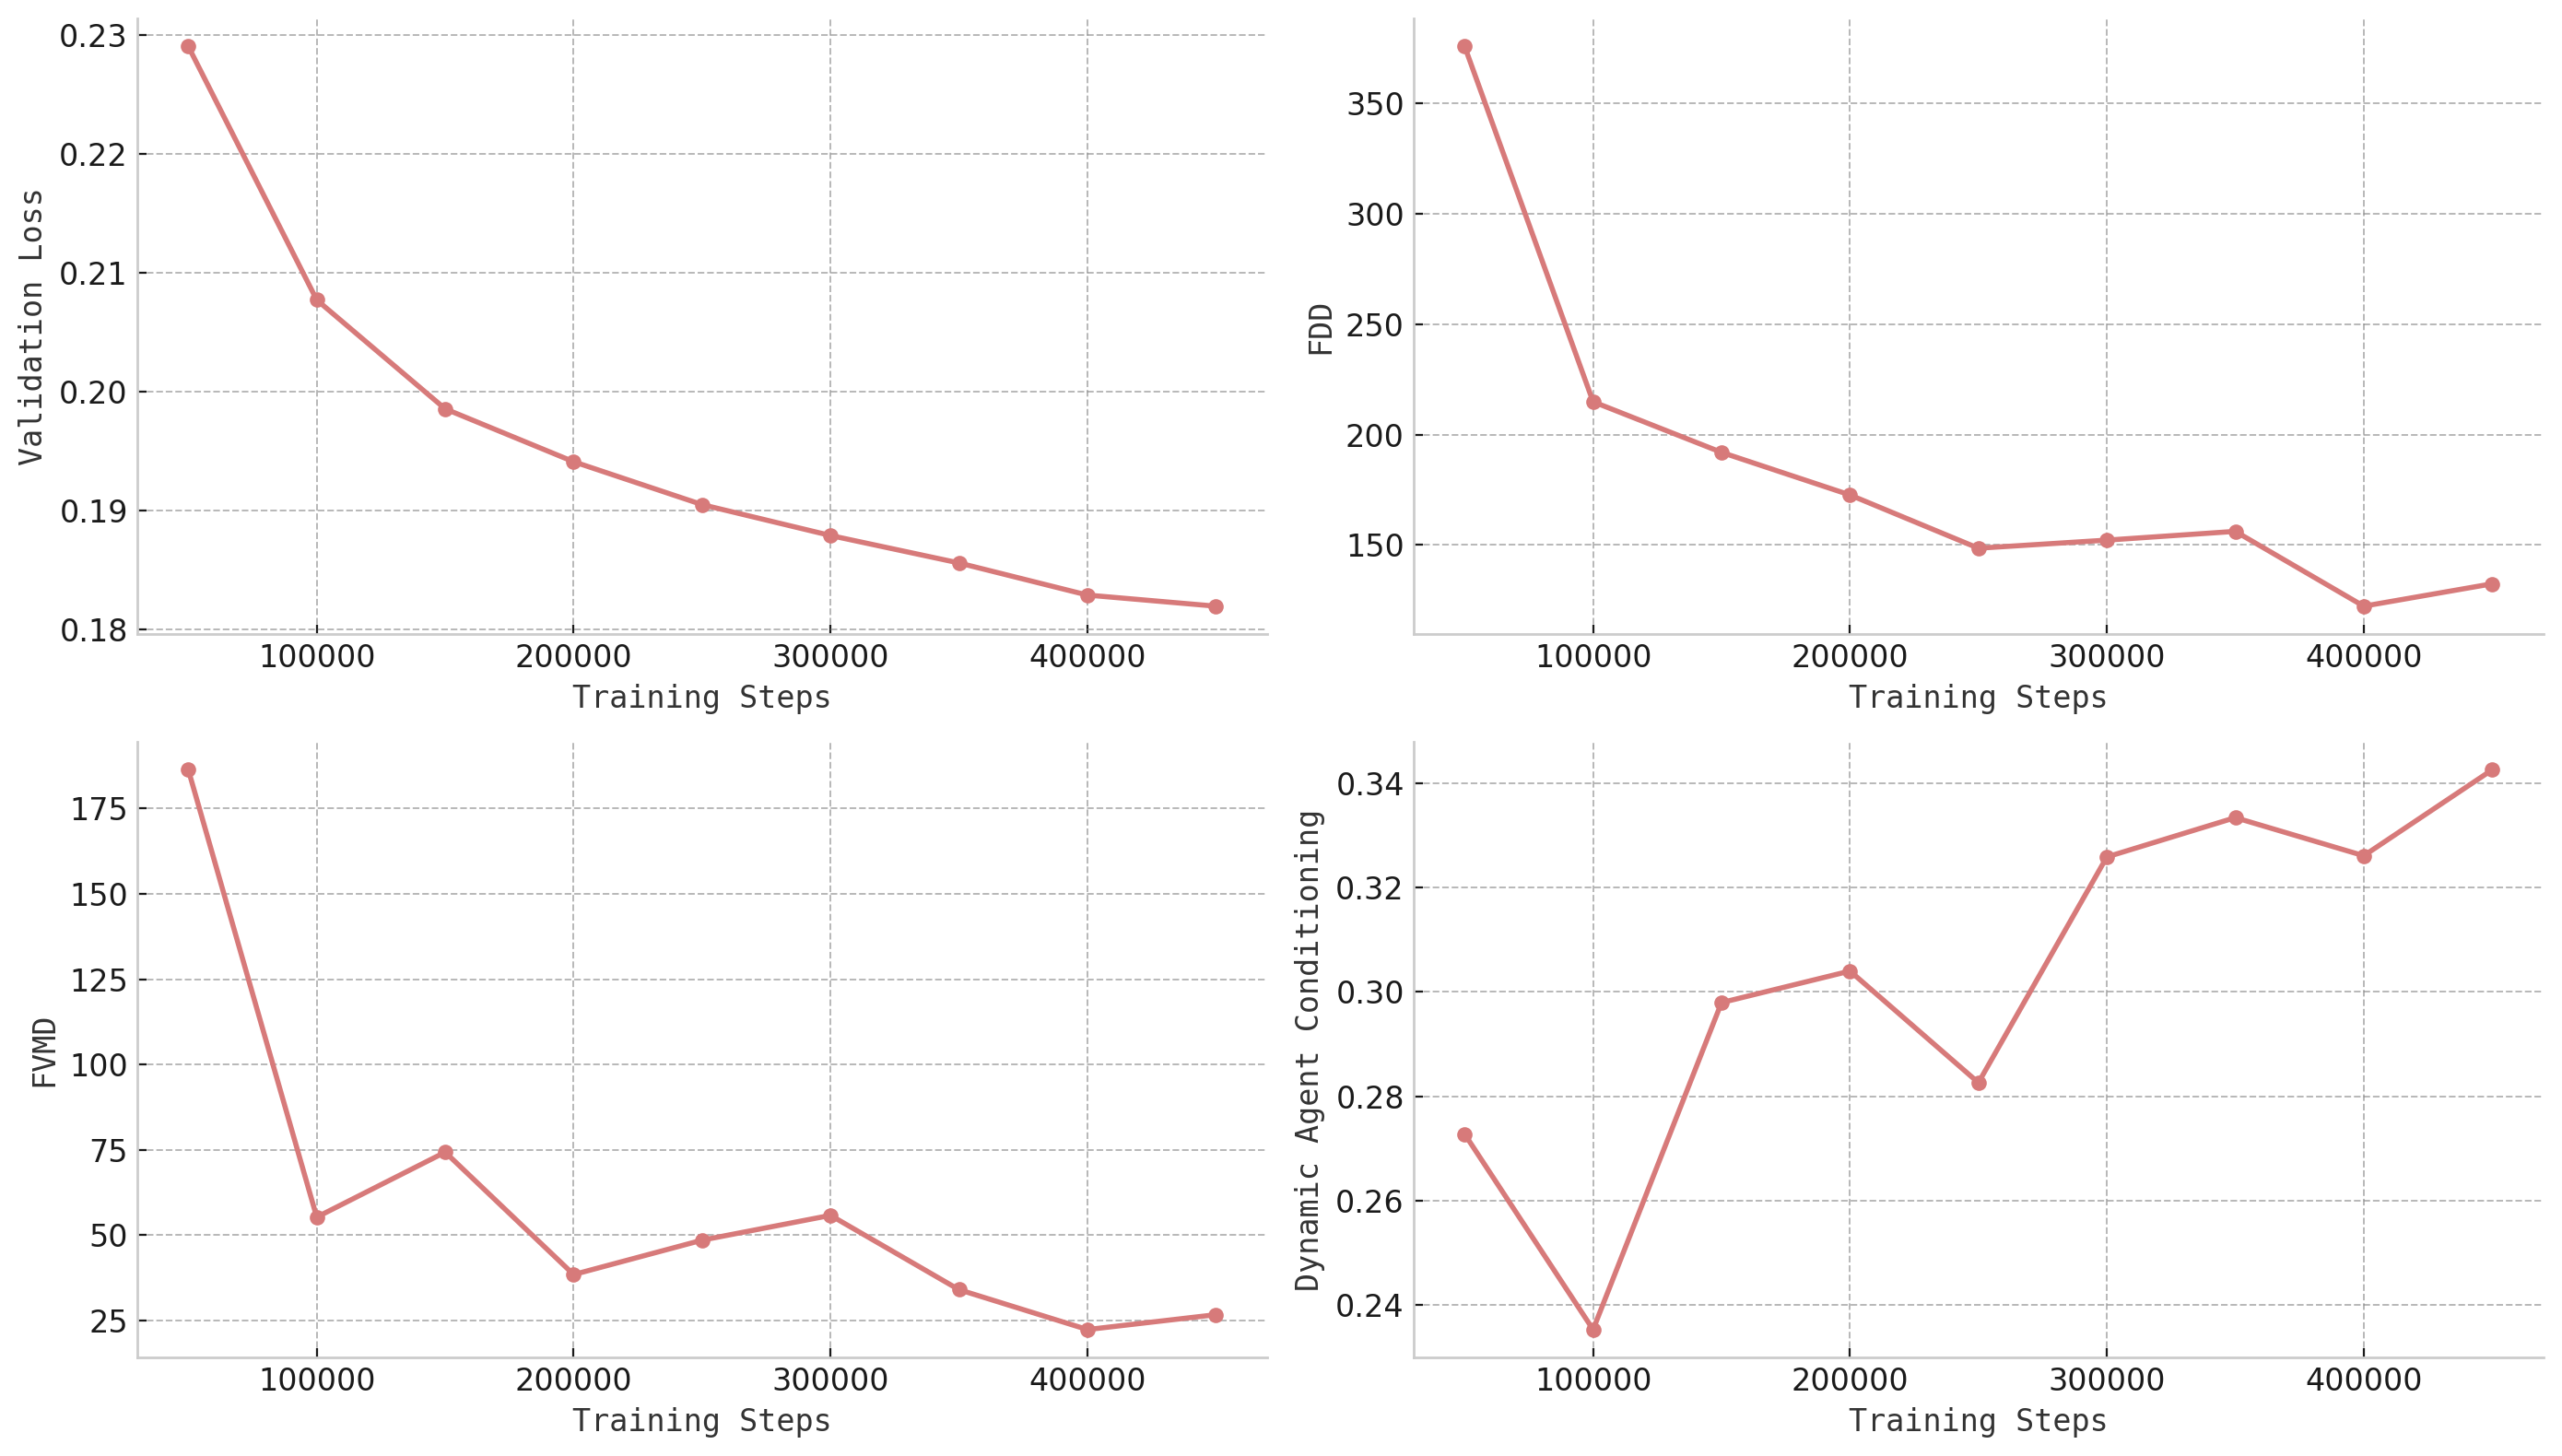
\includegraphics[width=1\textwidth]{Figures/metrics_v3.png}
    \caption{Validation loss and other metrics (evaluated on $n=1024$ samples). We found that the validation loss correlates well with human perceptual preferences.} 
    \label{fig:metrics}
\end{figure}

\paragraph{Dynamic Agent Conditioning.}  We evaluate dynamic agent fidelity by comparing the projection of the 3D bounding boxes (our conditional signal) with segmentation masks obtained via OneFormer \cite{jain2022oneformertransformerruleuniversal} on the generated video. We then compute class-based Intersection-over-Union (IoU) to measure how well the model adheres to the spatial and categorical specifications of dynamic agents during generation.

% \paragraph{Dynamic Agent Conditioning.} We evaluate dynamic agent fidelity by comparing 2D bounding boxes from generated videos with class-matched segmentation masks obtained via OneFormer~\cite{jain2022oneformertransformerruleuniversal}. Intersection-over-Union (IoU) is computed to assess how well the model adheres to the spatial and categorical specifications of dynamic agents during generation.

% \paragraph{Metadata conditioning.} To evaluate various metadata conditioning like weather, time of day, number of lanes, presence of zebra crossing etc., we train small logistic regression classifiers on top of CLIP \cite{radford21} embedding. We then compute average probability of class given in conditioning over frames of N video samples. We find that while these classifiers work well for global features like weather, they struggle to distinguish small differences in scene like traffic light state. 

We report the metrics and the validation loss in \Cref{fig:metrics}. The validation loss and other metrics are evaluated on the generation from scratch task with $n=1024$ samples. Despite some noise from small sample size, all metrics exhibit a positive trend throughout training. Notably, the validation loss shows the strongest correlation with human preference, making it a valuable proxy for perceptual quality.
